%!TEX TS-program = xelatex
%!TEX encoding = UTF-8 Unicode

De acuerdo a lo especificado en la consigna, para cada valor de densidad, siguiendo  el procedimiento propuesto por Alexander-Bloch y colaboradores (Alexander-Bloch et al., 2012). Para cada par NX y W se calcula la similaridad entre grupos a partir de Índice de Rand Ajustado (adjusted-for-chance Rand index, ARI), y el valor promedio se compara con Np permutaciones de las etiquetas de comunidades para cada estadío. El p-valor se obtiene dividiendo el número de veces en que una permutación supera el valor promedio para los datos no permutados por el número total de permutaciones (Np).

El valor obtenido para cada densidad se compara con los que se obtienen de realizar 300 permutaciones de las membresías de uno de los estadíos. 

Se observan los resultados del p-valor con un $+$ en cada una de las figuras.


\begin{figure}[H]
    \centering
    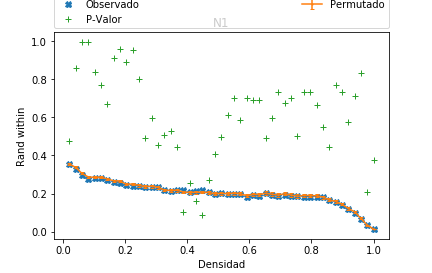
\includegraphics[width = 5in]{img/4_N1.png}
    \caption{N1}
    \label{fig:4_N1.png}
\end{figure}

\begin{figure}[H]
    \centering
    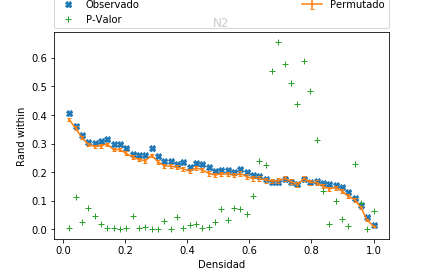
\includegraphics[width = 5in]{img/4_N2.png}
    \caption{N2}
    \label{fig:4_N2.png}
\end{figure}

\begin{figure}[H]
    \centering
    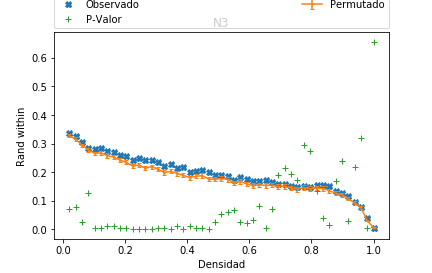
\includegraphics[width = 5in]{img/4_N3.png}
    \caption{N3}
    \label{fig:4_N3.png}
\end{figure}


Como conclusion de estos analisis podemos enunciar que las mayores diferencias en las membresías con respecto al estado \textbf{despierto} se registran en 
El estadío \textbf{N2} donde el índice de Rand inicia cerca del 0.4 y culmina muy cercano a 0 a medida que aumenta la densidad.

Destacamos que tanto en el estadío \textbf{N2} como el \textbf{N3}  se obtienen p-valores  significativos (0.05) lo cual no ocurre para el estadio \textbf{N1}.
No se observa una diferencia significativa entre los índices de Rand efectivos y los resultantes de las permutaciones.
